\documentclass{beamer}

\setbeamercovered{transparent}

\usepackage{pxfonts}
\usepackage{listings}
\title{Chapter 2: Number Systems and Codes
}
\subtitle{Lesson 1.1: Number Systems}
\author{Computer Fundamentals}
\institute{Second Edition}
 %\institute{\inst{1}Texas A\&M University \and \inst{2}Other University}
\date{\small{}}

% color
\definecolor{maroon}{RGB}{80,0,0} % A&M's primary color
\definecolor{332C2C}{RGB}{51,44,44} % A&M's primary support color, dark gray
\definecolor{5F574F}{RGB}{95,87,79} % A&M's secondary colors, light gray
\usecolortheme[named=maroon]{structure}
\setbeamercolor{frametitle}{fg=maroon,bg=white}
\setbeamercolor{primary}{fg=white,bg=maroon}
\setbeamercolor{secondary}{fg=white,bg=5F574F}

% headline
\setbeamertemplate{headline}{
\hbox{%
    \begin{beamercolorbox}[wd=0.5\paperwidth,ht=2.25ex,dp=1ex,left]{primary}
        \hspace*{2ex}\insertsectionhead % Section Title in Left
    \end{beamercolorbox}%
    \begin{beamercolorbox}[wd=0.5\paperwidth,ht=2.25ex,dp=1ex,left]{secondary}
        \hspace*{2ex}\insertsubsectionhead % Subsection Title in Right
    \end{beamercolorbox}}
\vskip0pt }

% footline
\setbeamertemplate{footline}{
\hbox{%
    \begin{beamercolorbox}[wd=.49\paperwidth,ht=2.25ex,dp=1ex,left]{primary}
        \hspace*{2ex}{Lesson 1.1: Introduction to Computers} % Something in Left
    \end{beamercolorbox}%
    \begin{beamercolorbox}[wd=.02\paperwidth,ht=2.25ex,dp=1ex,center]{primary}
        %\includegraphics[height=2.25ex,dp=2.25ex]{aTm08-box} % aTm Logo in the Middle
    \end{beamercolorbox}%
    \begin{beamercolorbox}[wd=.49\paperwidth,ht=2.25ex,dp=1ex,right]{primary}
        \insertframenumber{} / \inserttotalframenumber \hspace*{3ex} % Page numbers in Right
    \end{beamercolorbox}}
\vskip0pt }

\let\Tiny=\tiny



\begin{document}
\frame{\titlepage}

\section{Objectives}
\frame{
On completion of this lesson you will know:
\begin{itemize}
  \item Basic concepts of different number systems
\item	Characteristics of decimal, binary, octal and hexadecimal numbers
\item	Conversion of numbers

\end{itemize}
}
\section{Number Systems}
\frame
{In logical design, however, it is necessary to perform manipulations in the binary system of numbers because of the on-off nature of the physical devices used. The popular number systems are: 
\begin{itemize}
\item Decimal number system
\item Binary number system
\item Octal number system
\item Hexadecimal number system
\end{itemize}
}

\section{Number Systems}
\subsection{Decimal Number System}
\frame
{
It is the most commonly used number system in real life. It has the following features:
\begin{itemize}
\item	Digits: 0, 1, 2, 3, 4, 5, 6, 7, 8, 9  (total ten digits)
\item	Base (radix): 10 (ten)
\item	Weights: 1, 10, 100, 1000, � (powers of base 10)
\end{itemize}
}

\section{Number Systems}
\subsection{Decimal Number System}
\frame
{\frametitle{Example} Find the binary equivalent of the decimal number 1962.
\begin{figure}[ht!]
\centering
  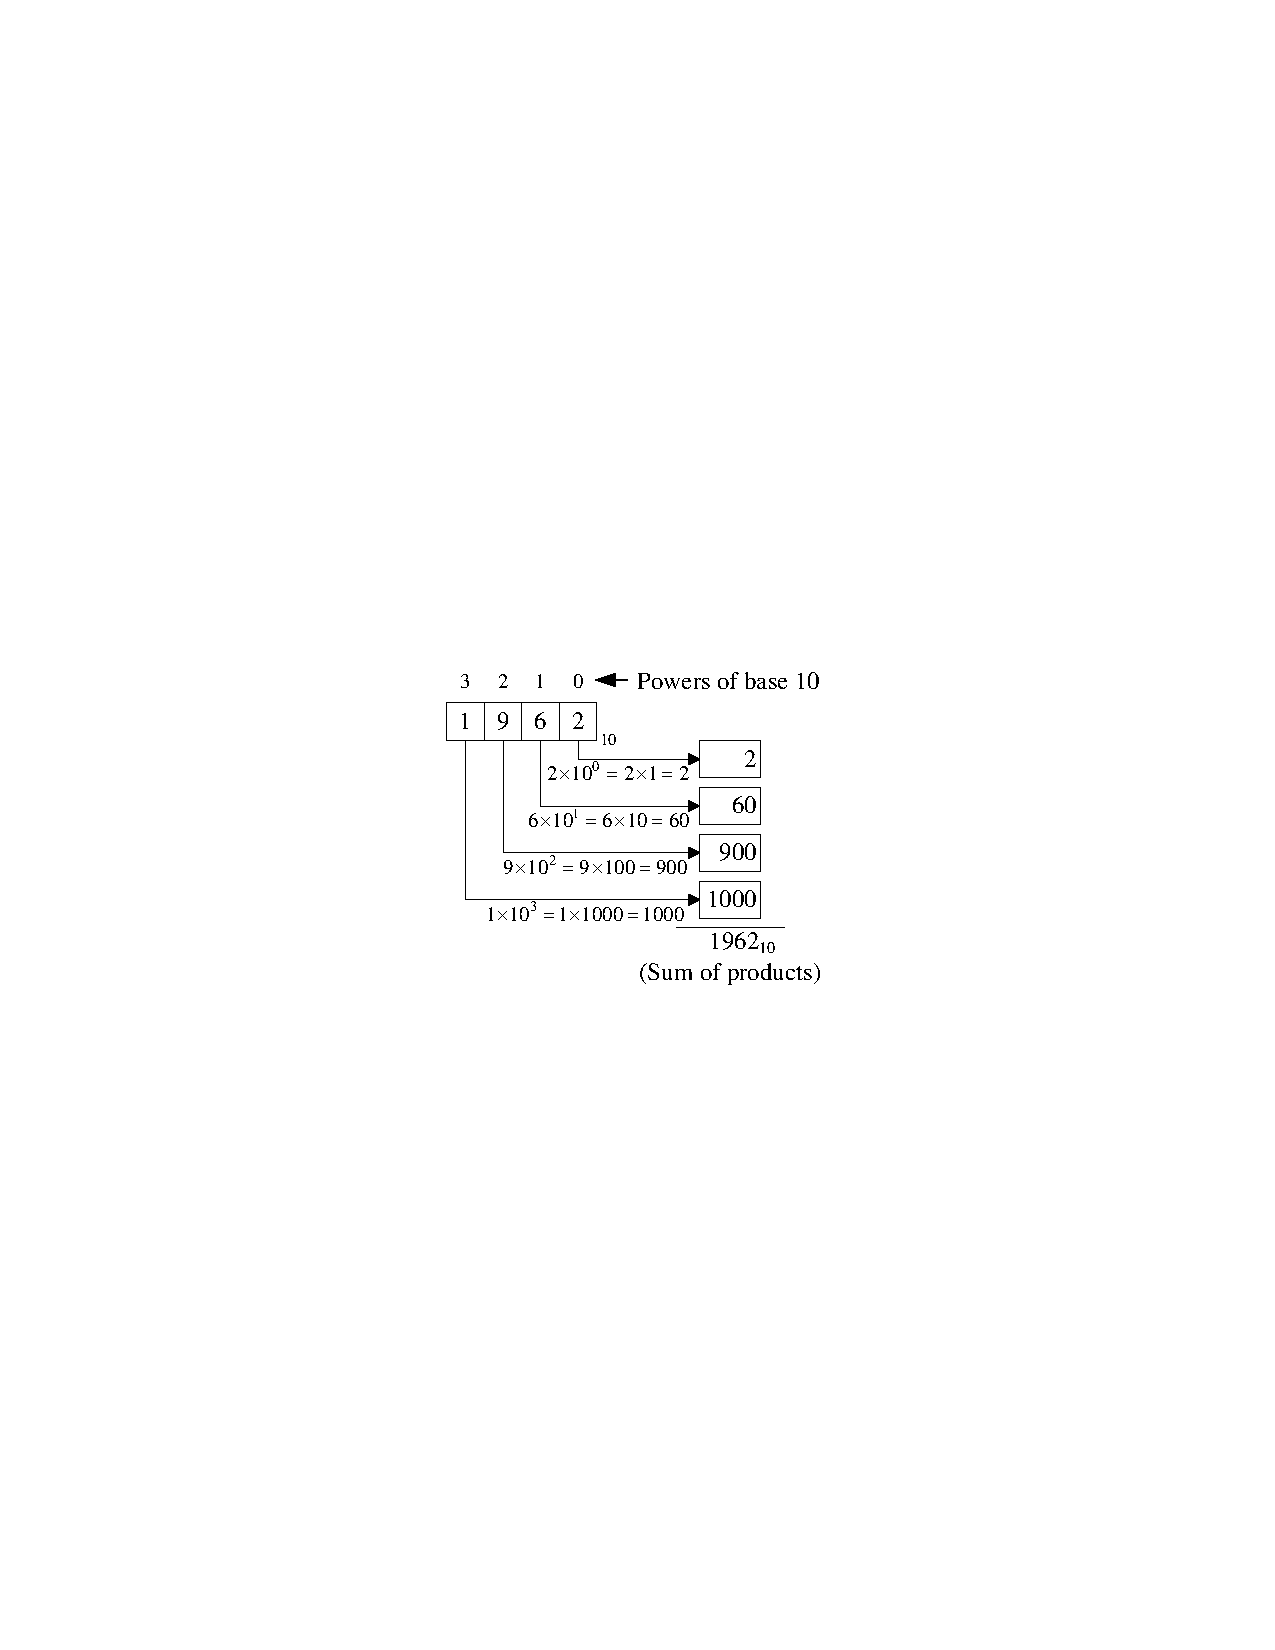
\includegraphics[width=8cm]{211}\\
  %\caption{1.1.1: Solving a program with a computer}
\end{figure}
}

\section{Number Systems}
\subsection{Decimal Number System}
\frame
{\frametitle{Example} Find the binary equivalent of the decimal number 1962.22.
\begin{figure}[ht!]
\centering
  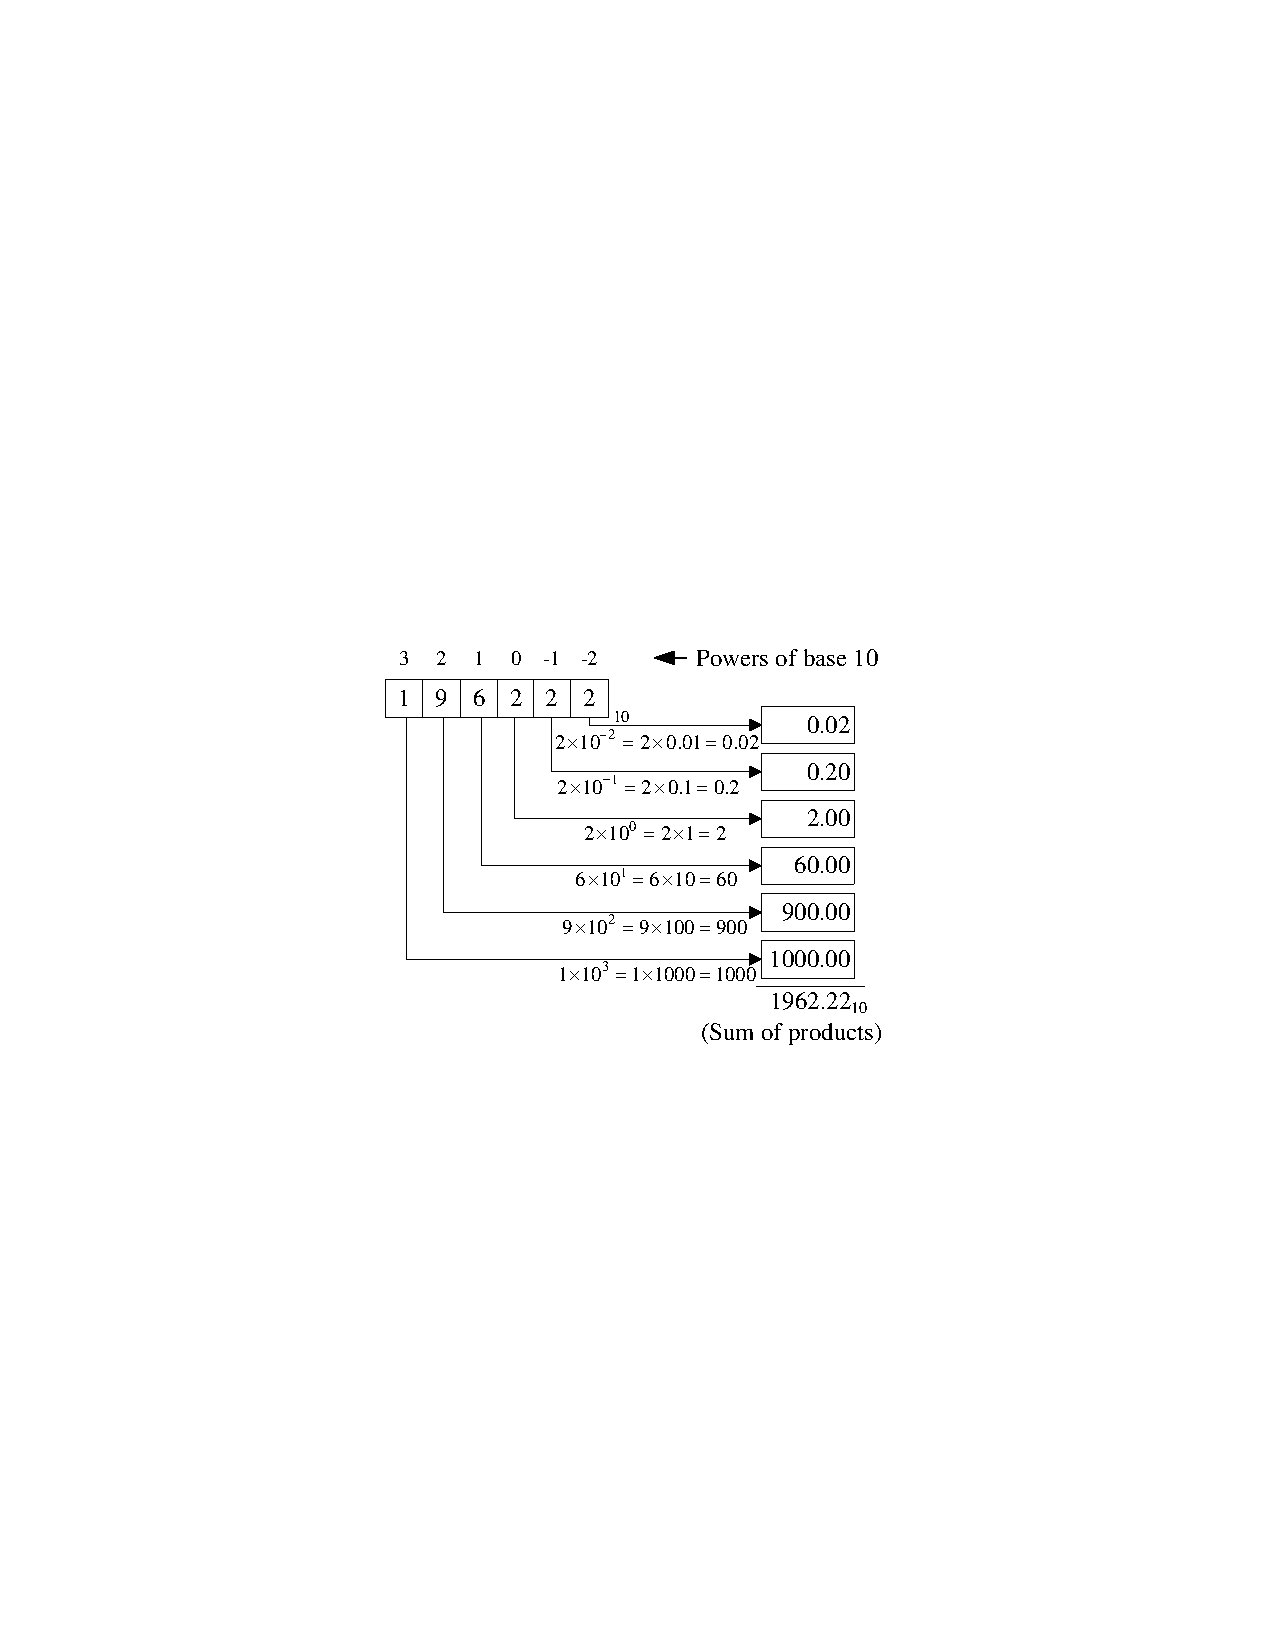
\includegraphics[width=8cm]{212}\\
  %\caption{1.1.1: Solving a program with a computer}
\end{figure}
}

\section{Number Systems}
\subsection{Binary Number System}
\frame
{Digital computers use binary numbers for internal operations. It has the following features:
\begin{itemize}
\item	Digits: 0, 1(total two digits)
\item	Base (radix): 2
\item Weights: 1, 2, 4, 8, 16, and so on (powers of base 2)
\end{itemize}
}

\section{Number Systems}
\subsection{Binary Number System}
\frame
{\frametitle{Example} Find the decimal equivalent of the binary 101011.
\begin{figure}[ht!]
\centering
  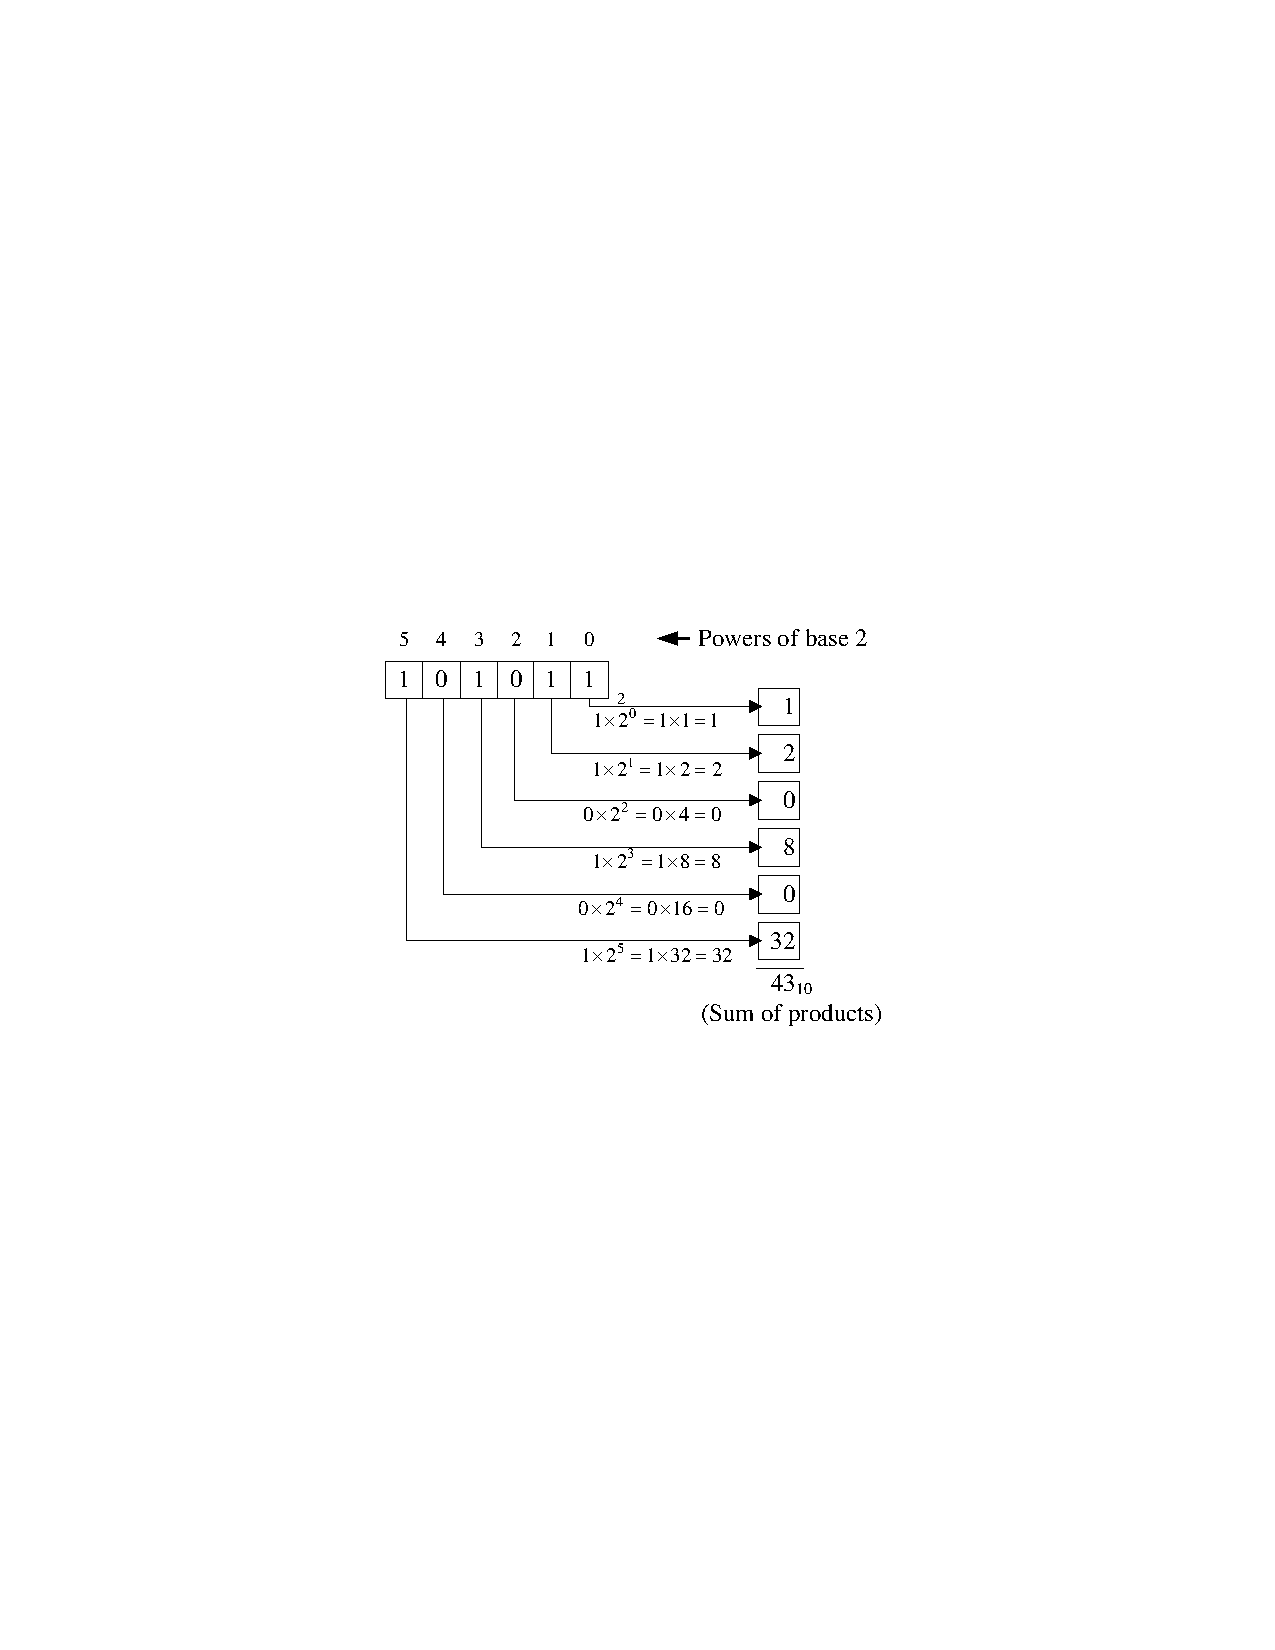
\includegraphics[width=8cm]{213}\\
  %\caption{1.1.1: Solving a program with a computer}
\end{figure}
}

\section{Number Systems}
\subsection{Octal Number System}
\frame
{Octal numbers are used in some programming languages. It has the following features:
\begin{itemize}
\item	Digits: 0, 1, 2, 3, 4, 5, 6, 7  (total eight digits)
\item	Base (radix): 8
\item Weights: 1, 8, 64, 512, and so on (powers of base 8)
\end{itemize}
}

\section{Number Systems}
\subsection{Hexadecimal Number System}
\frame
{Hexadecimal (also called hex in short) is a propositional numeral system. Hexadecimal is commonly used to represent computer memory addresses. It has the following features:
\begin{itemize}
\item	Digits: 0, 1, 2, 3, 4, 5, 6, 7, 8, 9, A, B, C, D, E, F  (total sixteen digits)
\item	Base (radix): 16
\item Weights: 1, 16, 256, and so on (powers of base 16)
\end{itemize}
}

\section{Converting from Decimal to base $r$ Systems}
\frame
{To convert a decimal number to its other equivalent numbers, the remainder method can be used. (This method can be used to convert a decimal number into any other base.) The remainder method involves the following four steps:
\begin{itemize}
\item Divide the decimal number by the base (in the case of binary, divide by 2).

\item Indicate the remainder to the right.
\item Continue dividing into each quotient (and indicating the remainder) until the divide operation produces a zero quotient.
\item The base 2 number is the numeric remainder reading from the last division to the first.
\end{itemize}
}

\section{Converting from Decimal to base $r$ Systems}
\frame
{\frametitle{Example 2.1.1 } Convert $47_{10}$ to its binary equivalent
\begin{figure}[ht!]
\centering
  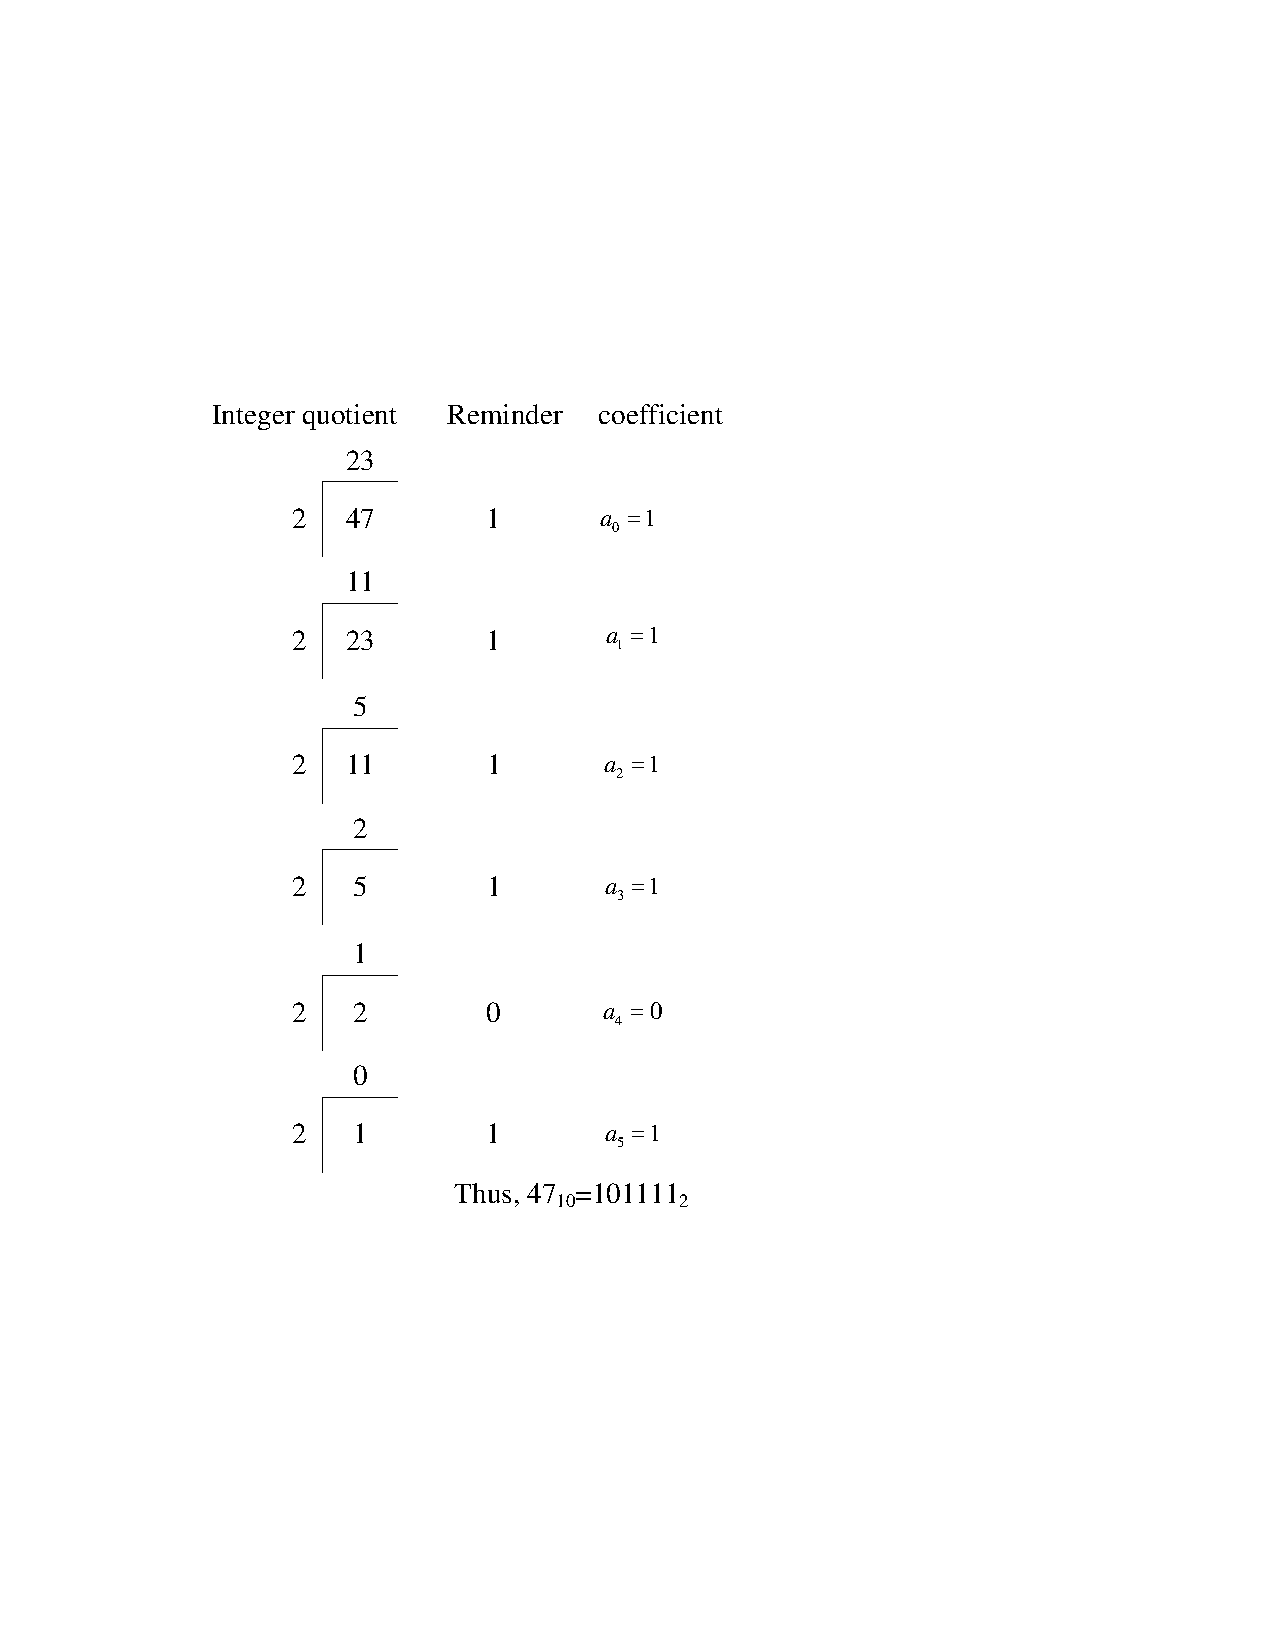
\includegraphics[width=4cm]{214}\\
  %\caption{1.1.1: Solving a program with a computer}
\end{figure}
}

\section{Converting from Decimal to base $r$ Systems}
\frame
{\frametitle{Example 2.1.2 } Convert $47_{10}$ to its octal equivalent
\begin{figure}[ht!]
\centering
  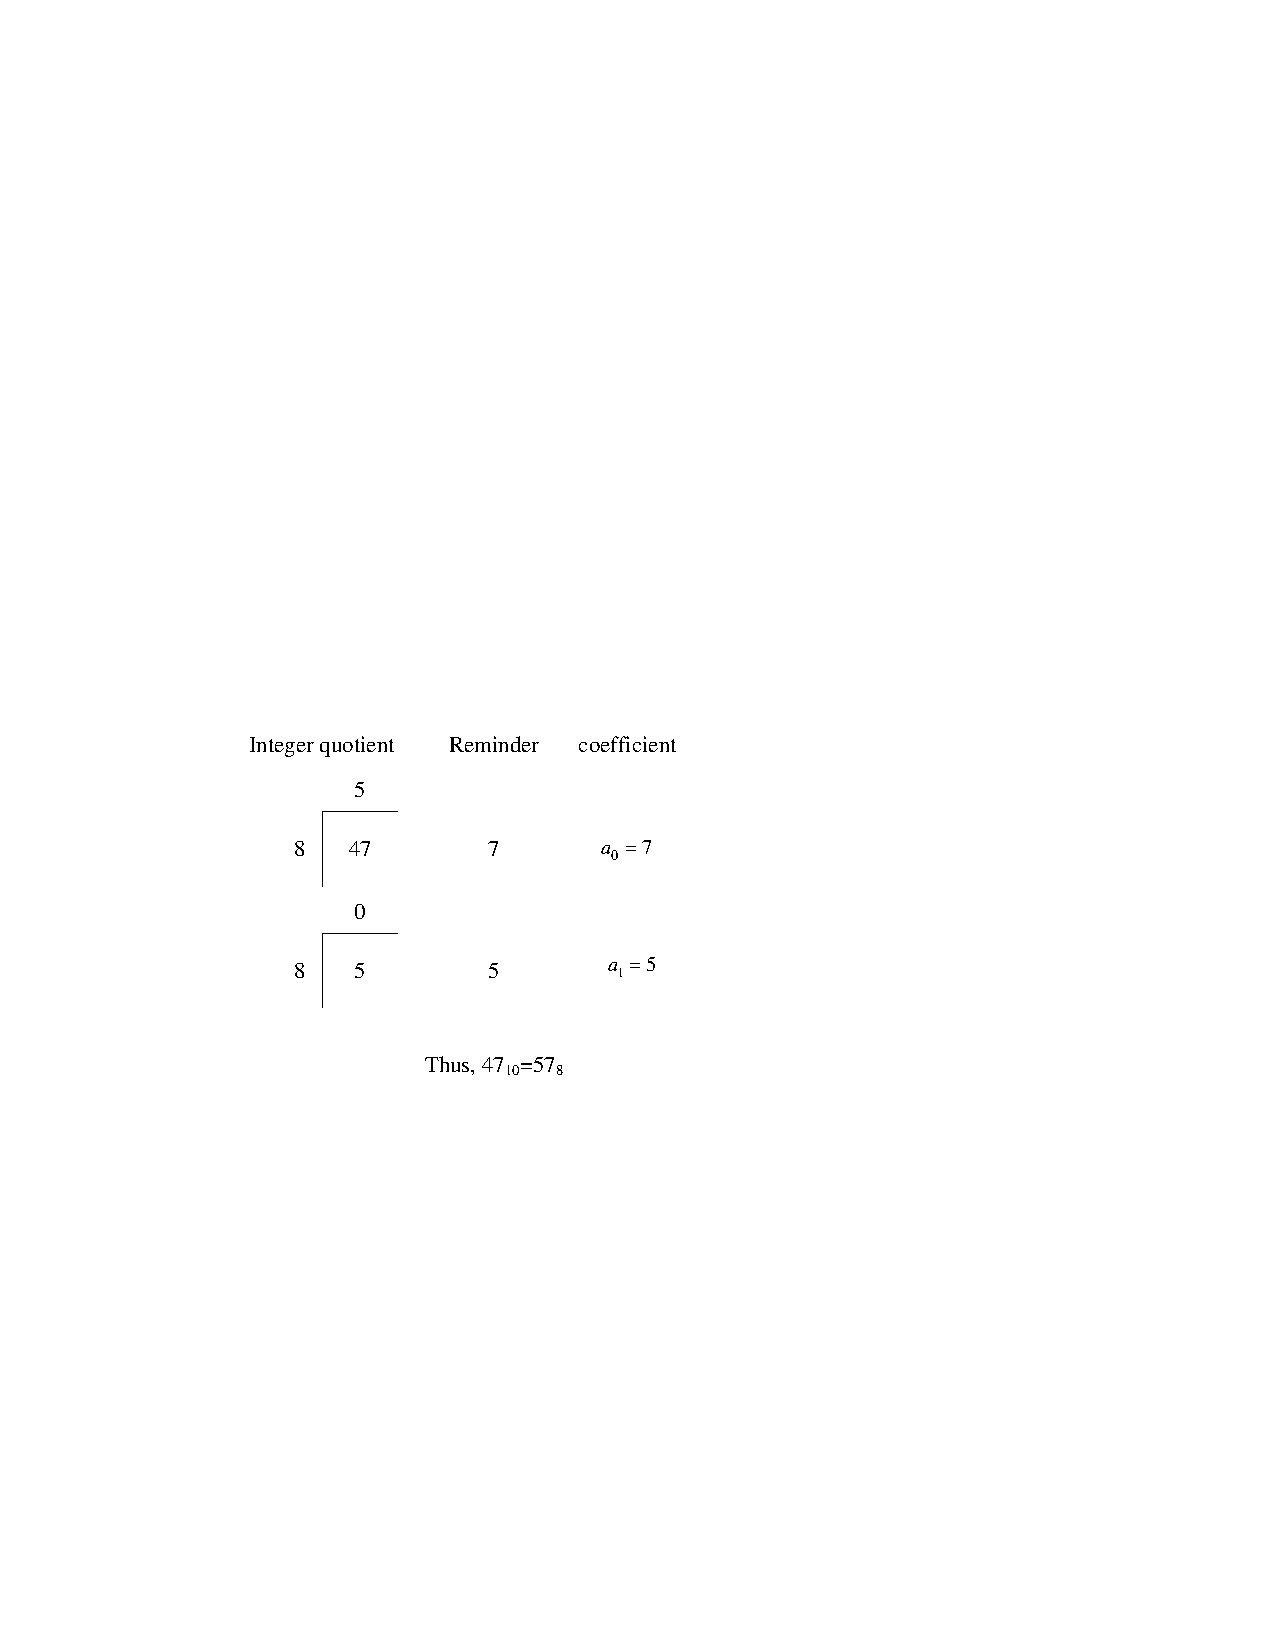
\includegraphics[width=6cm]{215}\\
  %\caption{1.1.1: Solving a program with a computer}
\end{figure}
}

\section{Converting from Decimal to base $r$ Systems}
\frame
{\frametitle{Example 2.1.3} Convert $47_{10}$ to its hexadecimal equivalent
\begin{figure}[ht!]
\centering
  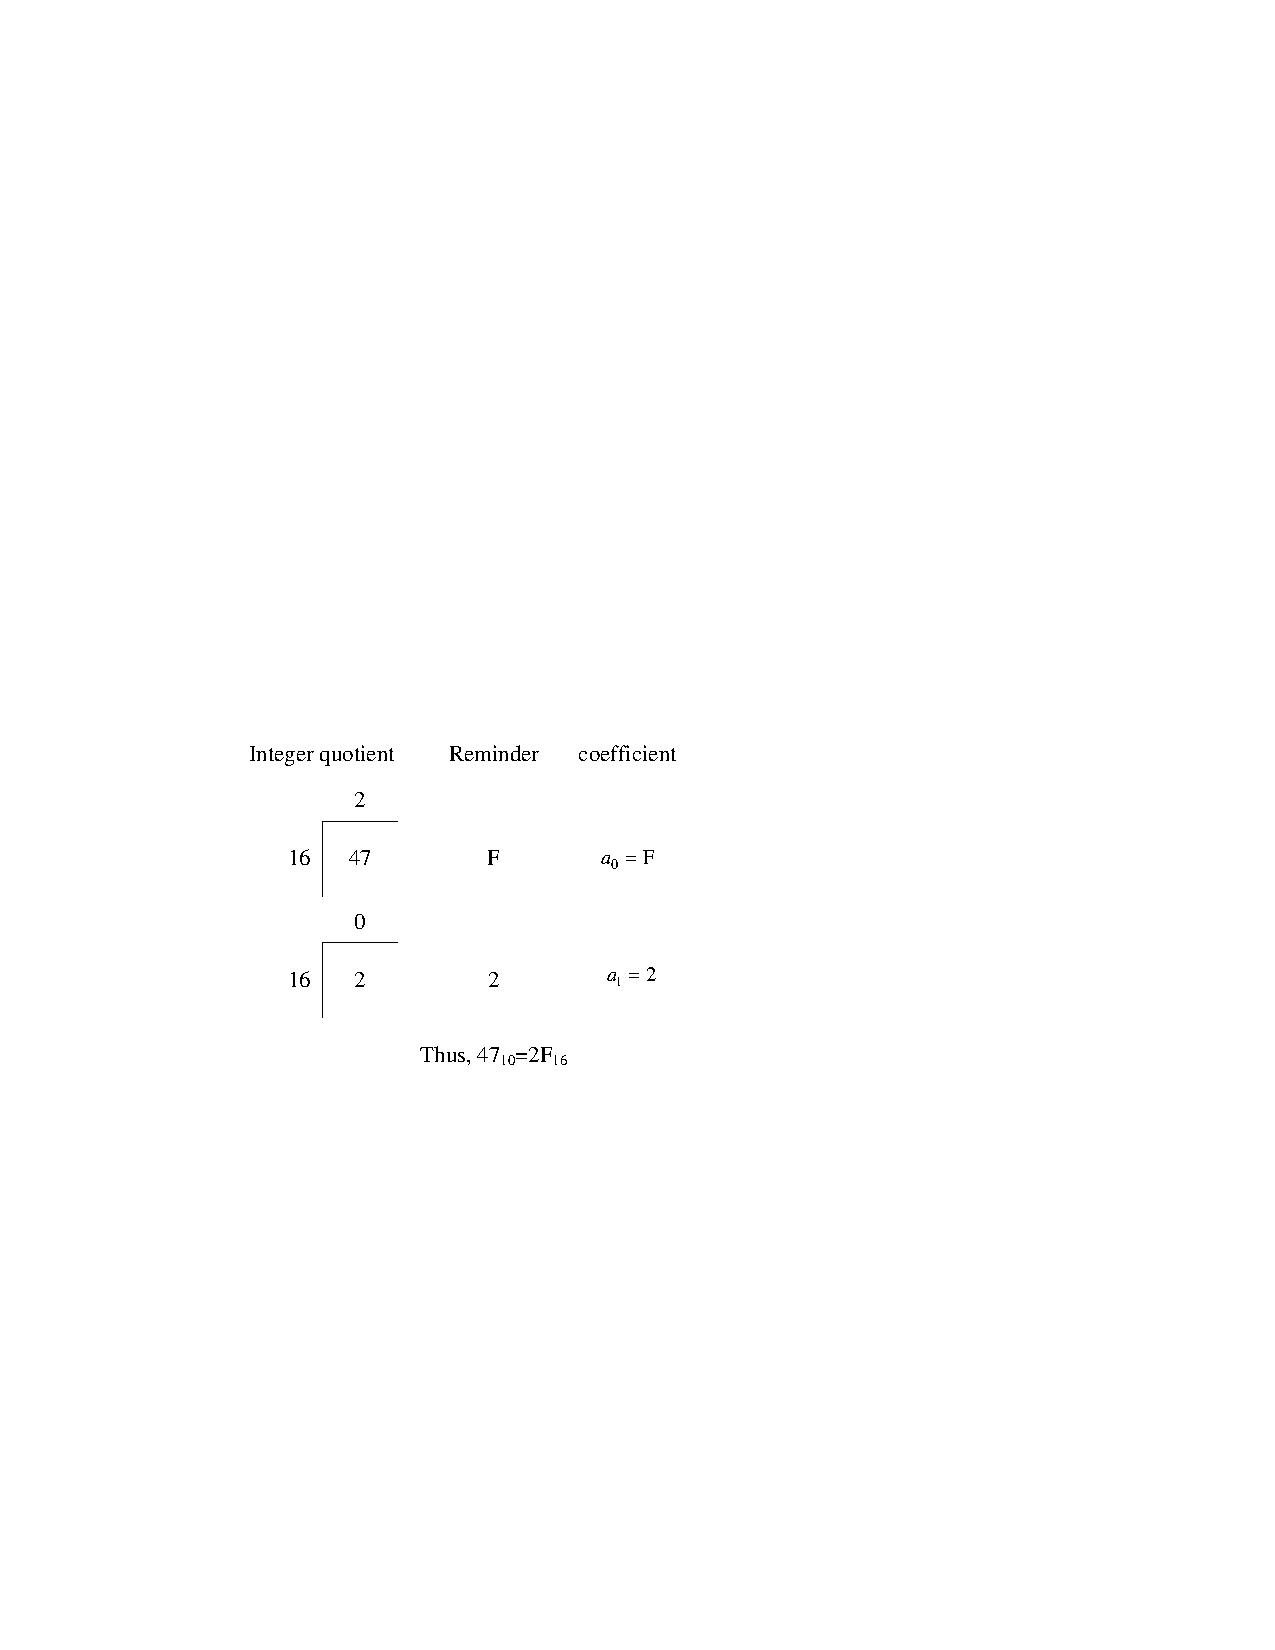
\includegraphics[width=6cm]{216}\\
  %\caption{1.1.1: Solving a program with a computer}
\end{figure}
}

\section{Converting from Decimal to base $r$ Systems}
\subsection{Binary to Octal: A Shortcut Method}
\frame
{The rule is as follows:
\begin{itemize}
\item	Starting from the right of the given binary stream into group of three, if leftmost group has fewer bits, attach the required number of leading 0s to complete the group.
\item	Determine equivalent octal digit for each group.
\end{itemize}
}

\section{Converting from Decimal to base $r$ Systems}
\subsection{Binary to Octal: A Shortcut Method}
\frame
{\frametitle{Example 2.1.4}
Find the octal number of $100110111_2$

Step 1:\\ $100$\;   $110$\;   $111$ \\
Step 2:\\ $100_2 = (1 \times 2^2) + (0\times 2^1) + (0\times 2^0)=4_8$ \\
$110_2 = (1 \times 2^2) + (1\times 2^1) + (0\times 2^0)=6_8$ \\
$111_2 = (1 \times 2^2) + (1\times 2^1) + (1\times 2^0)=7_8$ \\
Thus the octal number of $100110111_2$ is $467_8$
}

\section{Converting from Decimal to base $r$ Systems}
\subsection{Octal to Binary: A Shortcut Method}
\frame
{

The rule is as follows:
\begin{itemize}
\item	Find the equivalent binary group of 3 digits for each octal digit. 
\item	Find the results by combining binary groups
\end{itemize}

}

\section{Converting from Decimal to base $r$ Systems}
\subsection{Octal to Binary: A Shortcut Method}
\frame
{\frametitle{Example 2.1.5}
Find the binary number of $467_8$

Step 1:\\ $4_8=100_2$\;   $6_8=110_2$\;   $7_8=111_2$ \\
Step 2:\\ $100110111_2$ is the binary equivalent of $467_8$
}

\section{Converting from Decimal to base $r$ Systems}
\subsection{Binary to Hexadecimal: A Shortcut Method}
\frame
{

The rule is as follows:
\begin{itemize}
\item	Starting from the right of the given binary stream into group of four, if leftmost group has fewer bits, attach the required number of leading 0s to complete the group.
\item	Determine equivalent one hexadecimal digit for each group.
\end{itemize}
}

\section{Converting from Decimal to base $r$ Systems}
\subsection{Binary to Hexadecimal: A Shortcut Method}
\frame
{\frametitle{Example 2.1.6}
Find the hexadecimal equivalent number of $10011011_2$

Step 1:$1001$ \;   $1011$ \\
Step 2:\\$1001_2 = (1 \times 2^3) + (0\times 2^2) + (0\times 2^1)+(1\times 2^0)=9_{16}$\\
$1011_2 = (1 \times 2^3) + (0\times 2^2) + (1\times 2^1)+(1\times 2^0)=B_{16}$\\
Thus the binary number of $9B_{16}$ is $10011011_2$
}


\section{Converting from Decimal to base $r$ Systems}
\subsection{Hexadecimal to Binary: A Shortcut Method}
\frame
{

The rule is as follows:
\begin{itemize}
\item	Find the equivalent binary group of 4 digits for each hexadecimal digit. 
\item	Find the results by combining binary groups. 
\end{itemize}
}

\section{Converting from Decimal to base $r$ Systems}
\subsection{Binary to Hexadecimal: A Shortcut Method}
\frame
{\frametitle{Example 2.1.7}
Find the binary equivalent number of $9B_{16}$

Step 1: $9_{16}=1001_2$ \;   $B_{16}1011_2$ \\
Step 2: $10011011_2$ is the binary number of $9B_{16}$ is 
}


\end{document}
